\documentclass[jou]{apa6}

\usepackage[american]{babel}

\usepackage{csquotes}
\usepackage[style=apa,sortcites=true,sorting=nyt,backend=biber]{biblatex}
\DeclareLanguageMapping{american}{american-apa}
\addbibresource{bibliography.bib}


%%%%%%%%%%%%%%%%%%%%%%%%%%%%%%%%%%%%%%%%
%% Discrete Structures
%% The start of RBS stuff
%%%%%%%%%%%%%%%%%%%%%%%%%%%%%%%%%%%%%%%%

% Working internal and external links in PDF
\usepackage{hyperref}
% Extra math symbols in LaTeX
\usepackage{amsmath}
\usepackage{gensymb}
\usepackage{amssymb}
% Enumerations with (a), (b), etc.
\usepackage{enumerate}

\let\OLDitemize\itemize
\renewcommand\itemize{\OLDitemize\addtolength{\itemsep}{-6pt}}

\usepackage{etoolbox}
\makeatletter
\preto{\@verbatim}{\topsep=3pt \partopsep=3pt }
\makeatother

% These sizes redefine APA for A4 paper size
\oddsidemargin 0.0in
\evensidemargin 0.0in
\textwidth 6.27in
\headheight 1.0in
\topmargin -24pt
\headheight 12pt
\headsep 12pt
\textheight 9.19in



\title{Sample Quiz 4}
\author{Discrete Structures, Spring 2020}
\affiliation{RBS}

\leftheader{Discrete Sample Quiz 7}

\abstract{%
}

%\keywords{}

\setlength\parindent{0pt}

\begin{document}

%\thispagestyle{empty}

\twocolumn
\section{Worksheet 7: Counting}

\vspace{10pt}
{\bf Question 1 (Traversing Rubik's Cube).} A tiny ant wants to travel 
between two opposite vertices of a $3 \times 3 \times 3$ cube (Figure~\ref{fig:rubiks-cube}). It can crawl
on the surface of the cube (and even inside it); 
but any path should consist from exactly $9$ unit-length
steps, where each step is parallel to one of the coordinate axes ($x$, $y$ or $z$). 
Find the number of paths that the ant could take as it crawls from the vertex $A$ to the vertex $B$. 

\begin{figure}[!htb]
\center{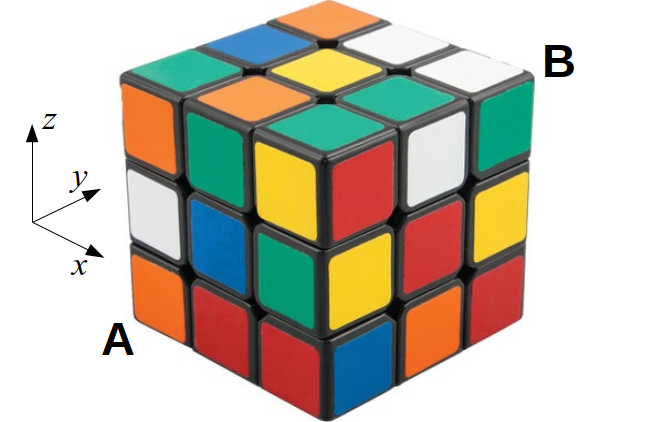
\includegraphics[width=2in]{quiz-sample-07/rubiks-cube.png}}
\caption{\label{fig:rubiks-cube} Rubik's cube.}
\end{figure}


Write your answer as an integer number equal to the number of paths from $A$ to $B$ satisfying the condition.






\vspace{6pt}
{\bf Question 2 (Permutations with Repetition).}\\
{\bf (A)} Find the number of ways (denoted by $N$) one can arrange the letters in the 6-letter word {\tt OLIVIA}. 
Both letters "I" are not distinguishable (if they switch places, it is still the same arrangement).\\
{\bf (B)} Assume that somebody writes out all the permutations of the word {\tt OLIVIA} 
in the {\em lexicographic ordering} (ordered as in a dictionary: sorted by the 1st letter; 
if the 1st letter is the same, then by the 2nd letter, etc.).\\
For example, the first permutation: $w_1 = \mathtt{AIILOV}$ and the last one is $w_N = \mathtt{VOLIIA}$. 
Find the permutations $w_{60},w_{61},w_{62},w_{63}$. 

Write your answer as a comma-separated list (first the total number of permutations, then the
$60$th,$61$st,$62$nd,$63$rd permutation).\\
$N$,$w_{60},w_{61},w_{62},w_{63}$. 


\vspace{6pt}
{\bf Question 3 (Raising to a high power).} 
Joe wrote the decimal notation of the following number:
$$X = \left( 10^{10} + 1 \right)^{10}.$$
After that, Joe erased the last $50$ digits of the number $X$, and got the number $Y$. 
Finally, Joe erased all the digits of $Y$, except the last ten digits, and got a sequence of digits $Z$.\\
{\bf (A)} Write all the digits of $Z$ (if it has leading zeroes, write them as well).\\
{\bf (B)} Express $Z$ as $C_n^k$ (``$n$ choose $k$''), where $k \leq n$.

Write your answer like this:\\ {\tt dddddddddd,choose(n,k)}.


\vspace{6pt}
{\bf Question 4 (Combinations with Repetition).} You have unlimited number of jellybeans \textendash{}
they can have any of these four colors: red, orange, green, yellow. The jellybeans of each
color are identical. Solve the following: express your answers as a binomial coefficients "$n$ choose $k$", 
where $k \leq n$.

{\bf (A)}  How many collections of $20$ jellybeans can you make? (The order of jellybeans in the collection 
does not matter. Those jellybean collections that have the same number of each color are considered identical.)\\
{\bf (B)} How many collections of $20$ jellybeans can you make, if there has to be at least one jellybean 
of each color. 

Write your answer in a form:\\ {\tt choose(n1,k1),choose(n2,k2)}\\
Replace {\tt n1,k1,n2,k2} with appropriate integers.


\vspace{6pt}
{\bf Question 5 (Ordering your combinations).} 
Somebody has written out all the combinations, how to choose $k=4$ months out of a set of 
$n=12$ months:\\
{\small
$\{ \mathtt{JAN},\mathtt{FEB},\mathtt{MAR},\mathtt{APR},\mathtt{MAY},\mathtt{JUN},
\mathtt{JUL},\mathtt{AUG},\mathtt{SEP},\mathtt{OCT},\mathtt{NOV},\mathtt{DEC} \}.$
}

All these four-month combinations are written in a sorted (so that a month appearing earlier in a year is always
written first), and furthermore \textendash{} all these combinations are arranged in increasing order. 
Months are ordered in this way: $\mathtt{JAN} < \mathtt{FEB} < \ldots < \mathtt{DEC}$.\\
The very first combination of months is $\mathtt{JAN},\mathtt{FEB},\mathtt{MAR},\mathtt{APR}$, 
the last one is $\mathtt{SEP},\mathtt{OCT},\mathtt{NOV},\mathtt{DEC}$. 

Write a comma-separated list of the four-months that is in the $100$th place in this list. 


\vspace{6pt}
{\bf Question 6: Pennies and jars.} 
Assume that you have $50$ pennies and three jars (these jars are initially labeled $A$, $B$, and $C$). 

{\bf (A)} In how many ways can you put the pennies in the jars, assuming that the pennies and the jars are distinguishable?\\
{\bf (B)} In how many ways can you put the pennies in the jars, assuming that the pennies are identical, but jars are distinguishable?\\
{\bf (C)} Assume that we remove the labels ($A$,$B$,$C$) from the jars; and the jars become indistinguishable. 
In how many ways can you put the pennies in the jars, assuming that both the pennies and the jars are indistinguishable?

\vspace{6pt}
{\bf Question 7 (Necklace with colored beads).} Assume that we have a circular necklace with 
$2012$ equally spaced beads. Exactly $7$ of the beads are red, the remaining ones are white. 
How many necklaces there are? (Necklaces that is obtainable from each other by rotating the
circle by some angle $\frac{2\pi}{2012}k$ ($k = 1,\ldots,2011$) are considered identical.)

{\em Note.} A more general question was asked in CGMO (China Girls Mathematical Olympiad), 
see Problem 8, \url{https://bit.ly/2TcfHH5}. 


\newpage
\subsection{Answers}

\vspace{6pt}
{\bf Question 1} Answer: {\tt 1680}\\
Every unit move of the ant can be expressed by a letter $X,Y,Z$ (depending 
on its direction). There are altogether $9!$ ways to arrange 
nine letters. Since all three letters $X$ can be mixed in any order, we need
to divide by $3! = 6$. For the same reason we can also mix all three $Y$s and 
all three $Z$s. Ultimately, 

$$\frac{9!}{3!3!3!} = 1680.$$

\vspace{6pt}
{\bf Question 2} Answer: TBD\\

\vspace{6pt}
{\bf Question 3} Answer: TBD\\

\vspace{6pt}
{\bf Question 4} Answer: TBD\\

\vspace{6pt}
{\bf Question 5} Answer: TBD\\

\vspace{6pt}
{\bf Question 6} Answer: TBD\\

\vspace{6pt}
{\bf Question 7} Answer: TBD\\






\end{document}

